\section{Problem 2: triaxial test loading}\label{sec:example2}\noindent
\subsection{FE model setup}\noindent
The investigation focuses on a fundamental triaxial test setup with an axisymmetric soil sample confined between two parallel, rough platens. As shown in \Cref{fig: FEmodel-triaxialsetup}, the simulation models drained triaxial tests using pure displacement. The assumptions of rigid platens and soil homogeneity ensure consistent stress distribution throughout the model. The soil sample, with a radius of $R = 38$ mm and a height of $H = 140$ mm, replicates a standard triaxial sample size. A two-dimensional axisymmetric mesh with 1,330 elements was employed to simulate the soil, with each element being a 4-node axisymmetric quadrilateral (CAX4P) for pore/fluid stress. Boundary conditions were applied such that vertical and horizontal displacements at the model base were fixed ($u_y$, $u_x = 0$), and horizontal displacement was fixed along the line of symmetry ($u_x = 0$). A uniform downward displacement was incrementally applied to the top edge of the mesh, reaching a maximum of 10 mm, to simulate a strain-controlled triaxial test. This method is commonly used in Abaqus numerical simulations \parencite{helwany2007, Matthew2024}. The red dashed line representing the line of symmetry. The axisymmetric model is swept along the axis of symmetry to illustrate the 3D representation. 



The Modified Cam-Clay model, commonly used in soil mechanics, captures key clay behavior under stress \parencite{roscoe1968}. Analyses and simulations were performed using Abaqus FEA with an implicit integration scheme and the standard solver to address nonlinearity, employing the Newton-Raphson method for solution updates and convergence. Uncertain soil parameters, including $\lambda$, $\kappa$, $\mathsf{M}$, and OCR, were varied, with their ranges, units, and meanings listed in \Cref{table: input parameters}. The outputs of interest are reaction force, axial deformation, and radial deformation. To generate the dataset for metamodel training, the four governing parameters were sampled from uniform distributions and a factorial design of 340 Monte Carlo simulations was conducted using Latin hypercube sampling. A covariance of 0.85 was applied between $\kappa$ and $\lambda$ to account for their interdependence, following \parencite{Matthew2024,dawood2025}.

\begin{table}[htbp]
\centering
\caption{Priors for parameter variations}
\begin{tabular}{llll}
\hline
$x$        & $\mathcal{D}_x$                            & Unit & Physical meaning                                                                        \\ \hline
$\lambda$      & $\mathcal{U}$(0.01, 1) & --  & Logarithmic hardening modulus                                                              \\
$\kappa$ & $\mathcal{U}$(0.01,1) & --  & Logarithmic bulk modulus
                                                   \\
$\mathsf{M}$  & $\mathcal{U}$(0.5,1.4) & --  & Critical state ratio                                                                \\
$OCR$      & $\mathcal{U}$(40.0, 150.0) & --  & Overconsolidation ratio                                                   \\
\hline
\end{tabular}
\label{table: input parameters}
\end{table}

Three outputs were collected: (1) reaction forces, $\mathcal{G}^{(1)} \in \mathbb{R}^{8 \times 1}$, (2) axial deformation, $\mathcal{G}^{(2)} \in \mathbb{R}^{8 \times 71}$, and (3) radial deformations of the triaxial specimen, $\mathcal{G}^{(3)} \in \mathbb{R}^{8 \times 71}$. Each simulation consisted of 8 loading increments, resulting in a three-output tensor. Due to the inherent complexity of the Modified Cam-Clay model, the responses exhibit evident nonlinearity, as illustrated in Figure \ref{fig: priorpred}. The prior predictive distribution in panel (a) highlights the overall reaction force characteristics before metamodel construction and Bayesian calibration, while panels (b) and (c) show axial and radial deformations for a representative triaxial test. Since the last two results are vector-based, only one sample is presented here to illustrate the response, without displaying the full output uncertainty.

\begin{table}[t]
\centering
\caption{Neural network architecture and parameter counts for triaxial loading problem}
\label{tab:nn_architecture_small}
\small
\setlength{\tabcolsep}{5pt}
\begin{tabular}{lll r}
\toprule
Layer & Type & Output shape & Params \\
\midrule
Input & InputLayer & (None, 4) & 0 \\
Dense & Dense(50) & (None, 50) & 250 \\
Repeat & RepeatVector(8) & (None, 8, 50) & 0 \\
LSTM & LSTM(50), return\_seq & (None, 8, 50) & 20{,}200 \\
\midrule
\multicolumn{4}{c}{\textbf{Branch A: scalar output}} \\
\midrule
TD-Dense & TimeDistributed(Dense(50)) & (None, 8, 50) & 2{,}550 \\
Output-A & TimeDistributed(Dense(1)) & (None, 8, 1) & 51 \\
\midrule
\multicolumn{4}{c}{\textbf{Branch B: vector output (1)}} \\
\midrule
TD-Dense & TimeDistributed(Dense(71)) & (None, 8, 71) & 3{,}621 \\
TD-Reshape & TimeDistributed(Reshape) & (None, 8, 71, 1) & 0 \\
TD-Conv1D & TimeDistributed(Conv1D(1)) & (None, 8, 71, 1) & 4 \\
Output-B & Lambda (squeeze) & (None, 8, 71) & 0 \\
\midrule
\multicolumn{4}{c}{\textbf{Branch C: vector output (2)}} \\
\midrule
TD-Dense & TimeDistributed(Dense(71)) & (None, 8, 71) & 3{,}621 \\
TD-Reshape & TimeDistributed(Reshape) & (None, 8, 71, 1) & 0 \\
TD-Conv1D & TimeDistributed(Conv1D(1)) & (None, 8, 71, 1) & 4 \\
Output-C & Lambda (squeeze) & (None, 8, 71) & 0 \\
\midrule
\textbf{Total} &  &  & \textbf{32{,}851} \\
\bottomrule
\end{tabular}
\end{table}

\setcounter{figure}{9} 
\begin{figure}
\centering
 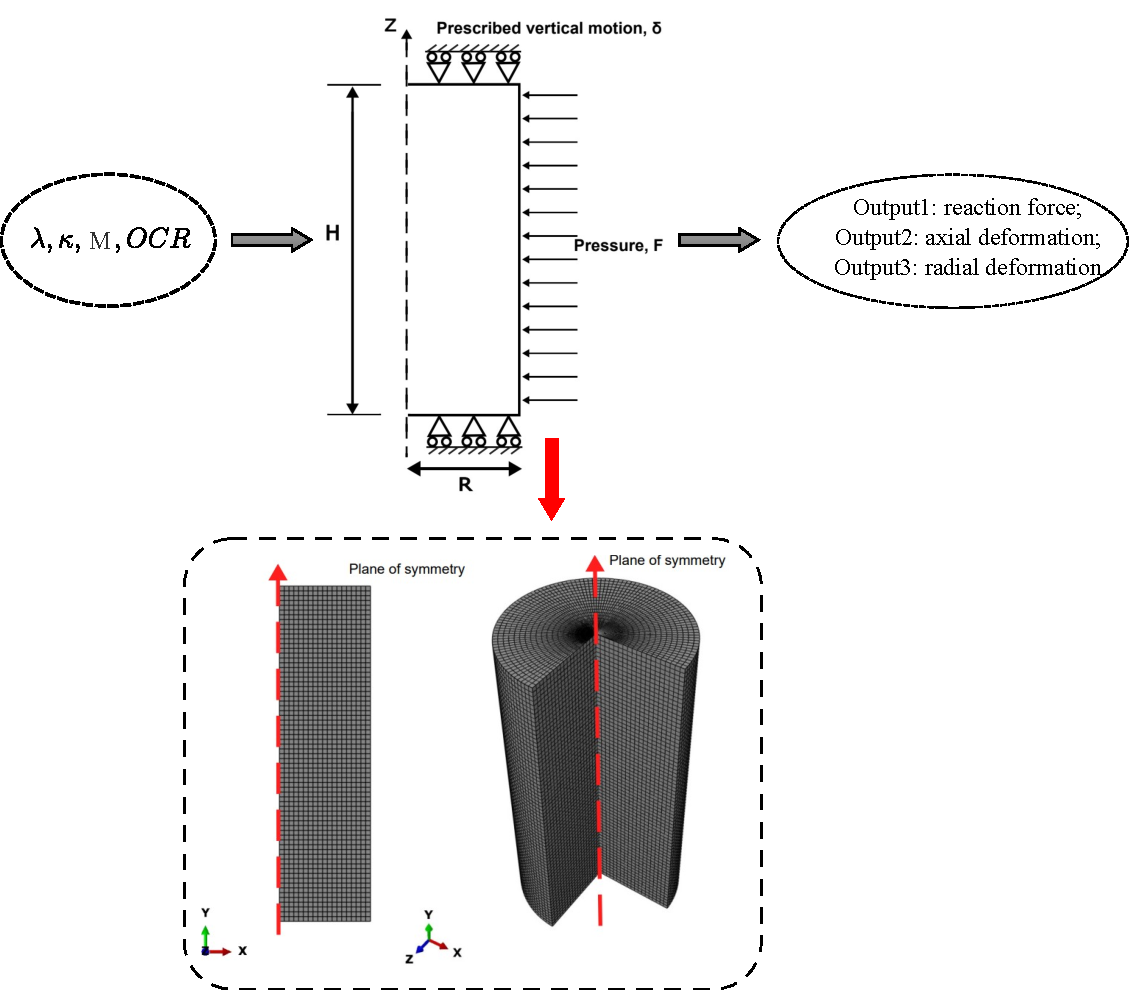
\includegraphics[width=140mm]{main_images/figure-FE-triaxial.pdf}
 \caption{Model setup}
 \label{fig: FEmodel-triaxialsetup}
\end{figure}
\begin{figure}
\centering
 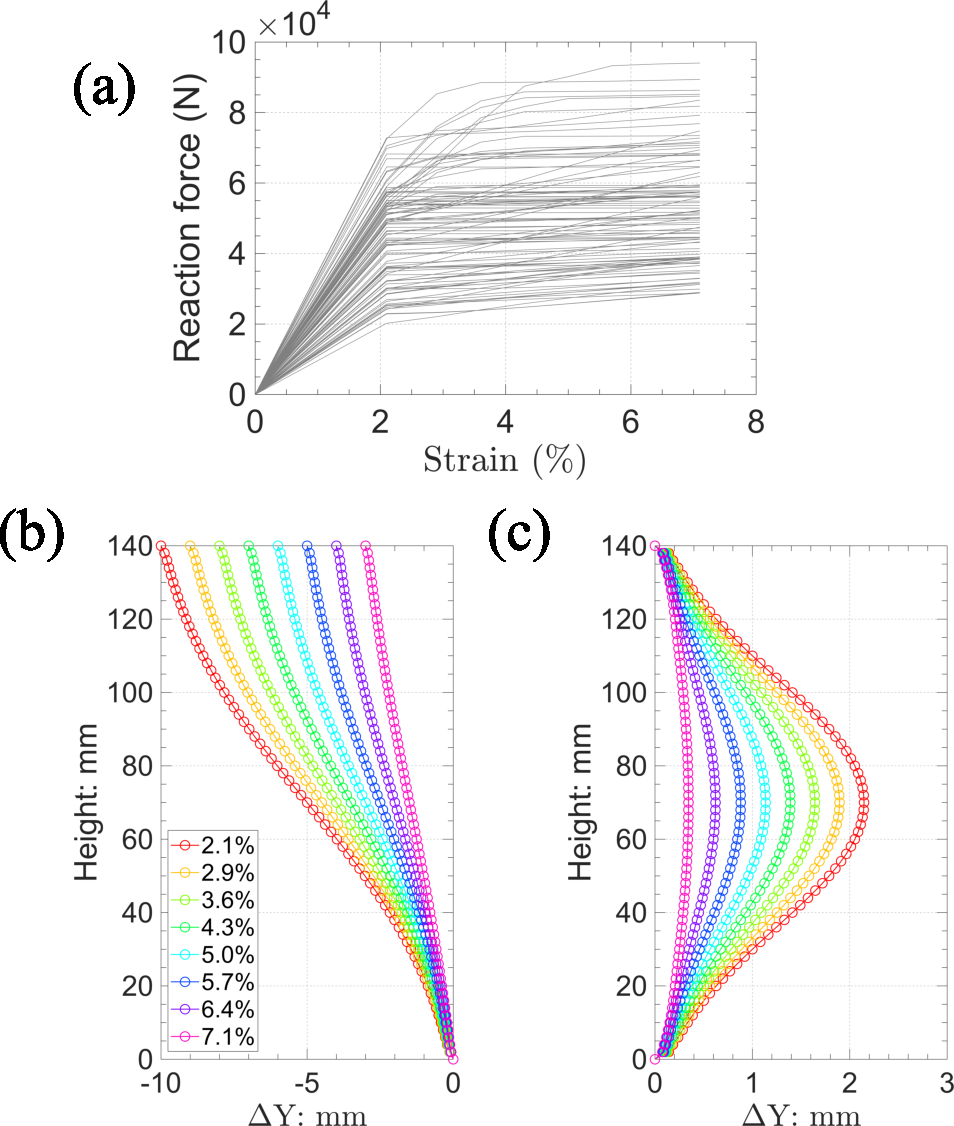
\includegraphics[width=90mm]{main_images/figure-priorpred.pdf}
 \caption{(a) Reaction force (prior predictive); (b) Axial deformation (one sample); (c) Radial deformation (one sample)}
 \label{fig: priorpred}
\end{figure}







\subsection{Metamodel construction}\noindent
80\% of the data are used for training and the remaining 20\% are reserved for testing. As shown in \Cref{tab:nn_architecture_small}, the model architecture consists of a multi-branch structure designed to predict three different outputs of the triaxial specimen. The network begins with an input layer that processes the input data into a latent feature space. This latent space is then passed through two dense layers, each with 50 hidden units, to learn meaningful representations of the input features. The resulting latent vector is then repeated across 8 loading increments, representing different loading stages, before being passed into an LSTM layer to capture temporal dependencies between these stages. The LSTM output is subsequently used as input for three distinct output branches. The first branch reconstructs the reaction forces ($\mathcal{G}^{(1)}$), with a shape of $\mathbb{R}^{8 \times 1}$, representing temporal force variations across 8 loading stages. This is achieved using time-distributed dense layers with 50 units, as there are no spatial features involved. The second branch reconstructs axial deformation ($\mathcal{G}^{(2)}$) with a shape of $\mathbb{R}^{8 \times 71}$, representing deformation across 8 stages and 71 mesh points. It uses a dense layer followed by three time-distributed transposed 1D convolution layers (kernel size 3, ReLU activation). The third branch, reconstructing radial deformation ($\mathcal{G}^{(3)}$), follows a similar approach to the second, utilising time-distributed transposed 1D convolutions to predict radial displacement over time.

\subsection{Likelihood configuration}\label{Likelihood configuration}\noindent
As shown in \Cref{eq: modified_Likelihood function}, the constructed surrogate model is embedded in the likelihood function $\mathcal{L}$ to accelerate the MCMC sampling. Since three different output types are considered, the total likelihood is taken as the product of three conditionally independent contributions,
\begin{equation}
\mathcal{L}_{\text{total}} = \mathcal{L}_{1} \times \mathcal{L}_{2} \times \mathcal{L}_{3},
\end{equation}
where $\mathcal{L}_{r}$ denotes the likelihood associated with the $r$-th output type. The observations are generated synthetically by perturbing the reference FE response with additive Gaussian noise of 3\%, so that a “ground-truth’’ data set is available and the corresponding soil parameters are known but not used either for training the surrogate model or within the MCMC procedure.

As discussed in \Cref{sec: SBI}, a Gaussian-type model is adopted for each output type. Although more elaborate or problem-specific likelihood formulations could be used, the Gaussian likelihood is chosen here for its simplicity and widespread use. For each output type $r$, the residual noise between surrogate predictions and observations is modelled as zero-mean Gaussian with diagonal covariance $\Sigma_{\varepsilon_r} = \sigma_r^{2}\mathbb{I}$. The variance $\sigma_r^{2}$ is treated as an additional unknown and inferred jointly with the soil parameters, with a weakly informative prior $\sigma_r \sim \mathcal{U}\bigl(0,\max(\mathcal{Y}_r)\bigr)$, where $\mathcal{Y}_r$ denotes the set of observations for output type $r$. This choice links the admissible noise level to the magnitude of the corresponding measurements. It should be noted that heteroscedastic noise is not modelled in this study, since only a single monitoring realisation is available and a more complex noise structure would not be identifiable in a robust manner; with richer monitoring data, heteroscedastic extensions could be introduced. All time steps and all three output types are assimilated through sequential Bayesian updating. The posterior distribution of the soil parameters and noise variances is approximated using an affine-invariant ensemble sampler with 300 chains of 300 steps each, discarding the initial 70\% of iterations as burn-in.


\subsection{Performance}\noindent
To assess the performance of the constructed metamodel, \Cref{fig: triaxialperformance} presents regression plots of predictions against reference values for both training and test datasets. The diagonal line indicates perfect agreement, and the results show good consistency. The metamodel was further evaluated within a sequential Bayesian inversion framework to test its ability to quantify uncertainty, a critical aspect in geotechnical applications. Following the procedure in \Cref{sec: SBI,Likelihood configuration}, the metamodel was embedded in the likelihood function to accelerate the inversion. One dataset sample was withheld as ground truth ($\lambda$ = 0.49, $\kappa$ = 0.06, $\mathsf{M}$ = 0.72 and $OCR$ = 130), excluded from both training and testing, and subsequently treated as synthetic observations for calibration. As shown in \Cref{fig: Cornerplot}, parameter uncertainty progressively decreases with additional observations, as expected. The predefined ground truth (black dashed lines) is approached by the posterior distributions (blue regions), with the MAP estimates (red circles) clustering closely around the true values, demonstrating the metamodel’s effectiveness in inversion. Together, these results confirm that the constructed metamodel provides both accurate predictions and reliable support for uncertainty quantification tasks.





\begin{figure}[htbp]
    \centering
    \begin{subfigure}[b]{\textwidth}
        \centering
        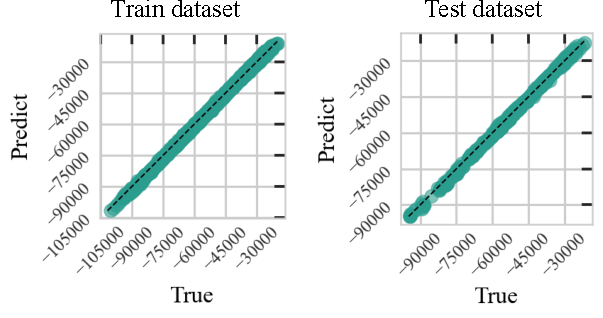
\includegraphics[width = 90mm]{main_images/figure-problem2-2.pdf}
        \caption{$\mathcal{G}^{(1)}$}
    \end{subfigure}%
    \vfill
    \begin{subfigure}[b]{\textwidth}
        \centering
        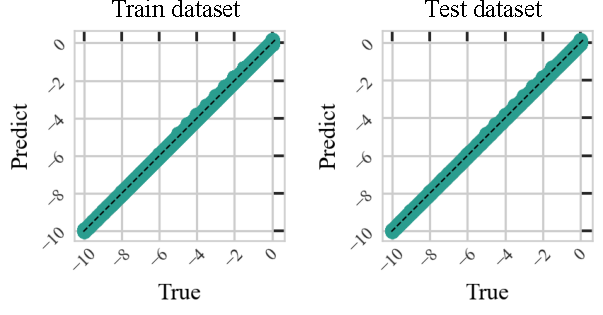
\includegraphics[width = 90mm]{main_images/figure-problem2-1.pdf}
        \caption{$\mathcal{G}^{(2)}$}
    \end{subfigure}%
    \vfill
    \begin{subfigure}[b]{\textwidth}
        \centering
        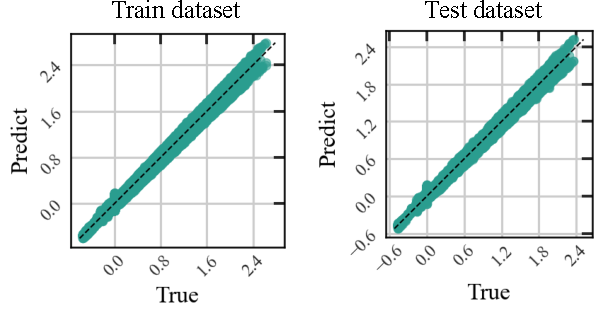
\includegraphics[width = 90mm]{main_images/figure-problem2-3.pdf}
        \caption{$\mathcal{G}^{(3)}$}
    \end{subfigure}%
    \caption{Triaxial metamodel performance: (a) Reaction force; (b) Axial deformation; (c) Radial deformation}
    \label{fig: triaxialperformance}
\end{figure}








\begin{figure}[htbp]
\centering
 \includegraphics[width=190mm]{main_images/figure-cornerplot.pdf}
 \caption{Corner plot for uncertain soil parameters}
 \label{fig: Cornerplot}
\end{figure}

% \begin{figure}[htbp]
% \centering
%  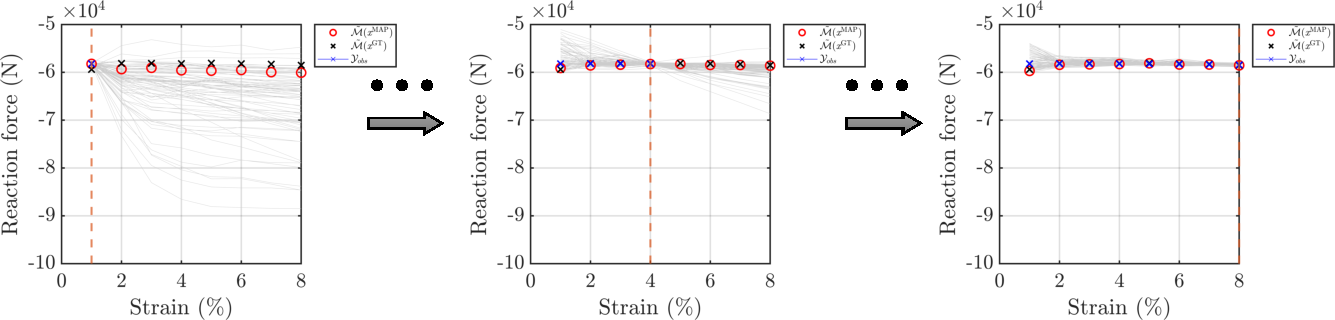
\includegraphics[width=140mm]{main_images/figure-UQ.pdf}
%  \caption{Uncertainty quantification process for reaction force}
%  \label{fig: UQ}
% \end{figure}